

\begin{frame}{OCaml 5}

 \subtt{Sortie de OCaml 5 à la rentrée}
    \begin{itemize}[label=\small\ding{114}]
        \item OCaml multicore
        \item les effets 
    \end{itemize}
\pause

\begin{figure}
    \centering
    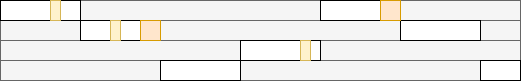
\includegraphics[width=0.9\textwidth]{slides/images/concurrence.png}
    \caption{Concurrence}
\end{figure}

\begin{figure}
    \centering
    \includegraphics[width=0.9\textwidth]{slides/images/parallélisme.png}
    \caption{Parallélisme}
\end{figure}
% Blanc = code OCaml
% Jaune = minor GC
% Orange = major GC
\end{frame}

\begin{frame}[fragile]{Effets}

\begin{lstlisting}
effect Compter : int

let programme () =
    let somme = ref 0 in
    for i = 0 to 9 do
        somme := !somme + perform Compter
    done;
    print_int !somme

let _ =
  let compteur = ref 0 in
  try programme () with
  | effect Compter k -> 
    incr compteur;
    Printf.printf "+1: %d\n" !compteur;
    continue k (!compteur)
\end{lstlisting}

    
\end{frame}